\label{chap:arch}

\begin{figure*}[ht] \centering
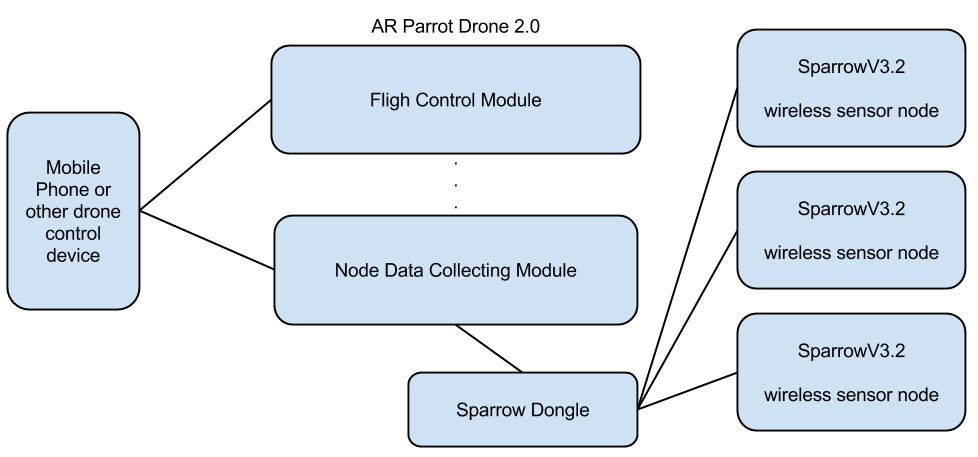
\includegraphics[width=0.7\textwidth]{img/organigrama.png}
\caption{Modules and connections between them and devices} \end{figure*}

The classic way of implementing a gateway is by using stationary devices or mobile devices like laptops or phones connected to at least one wireless node. The problem with this type of mobile devices is that you have to be in close proximity of the node in order to communicate with it. This might not be a problem if the nodes are easily accessible, but if a node is located in a remote location (e.g. at a high altitude or over a cliff, or even at an unknown location), using drones seems to be the best alternative.

Having this to say, our design has a number of features useful in everyday interaction with a wireless node outlined in \ref{sec:inter},\ref{sec:prox}. 

They can be launched from anywhere, fly to any place a node might be placed, gather all the information collected by the nodes and even air-drop nodes.

A number of design features were included for ease-of-use in
research and development, outlined in \ref{sec:eng},\ref{sec:data}.


\subsection{\textit{Ease of interaction}} 

\label{sec:inter}

The drone automatically detects and initiates a communication with a nearby node. It searches permanently for any signal emitted by a node and sends an acknowledgement packet back to it when it receives any signal. After this first handshake is complete, the node has green light to transmit the information to the gateway installed on the drone. If a node has been detected, the pilot is informed of its presence or if the data transaction completed successfully so that he may continue in the search for another node.

\subsection{\textit{Proximity function}} 

\label{sec:prox}

The SparrowDongle can supply informations regarding the nearby nodes by reading the strength of the received signal. Using this information, the pilot can direct the drone closer to the nodes location, either for a faster transfer or to find its exact location\cite{yedavalli2005ecolocation}. 

Besides the signal strength offered by the SparrowDongle, the drone features an on-board camera with a resolution of 1280x720 pixels streaming at 30 fps. This is very useful in pin-pointing the exact location of a wireless sensor node.


\subsection{\textit{Energy Saver}} 

\label{sec:eng}

Due to the communication protocol implemented, the SparrowV3.2 node uses very little power when not connected to the drone. It broadcasts just a small packet at fixed intervals for low consumption and enters a high bandwidth mode when it detects the presence of a drone for a fast data transfer, similar to the solution described by Cardei et al.  \cite{cardei2005improving}.

\subsection{\textit{Latest Data}} 

\label{sec:data}

The data is stored on the flash micro controller of the node. In this way, the data is persistent in the memory even the power drops and can be recovered when the power is restored. When the memory is full, the oldest data is deleted in order to make space for new one. The data sent to the drone is from the oldest to the newest, so that in the event of a connection lost the node has free space for new data. 


\begin{figure*}[ht] \centering
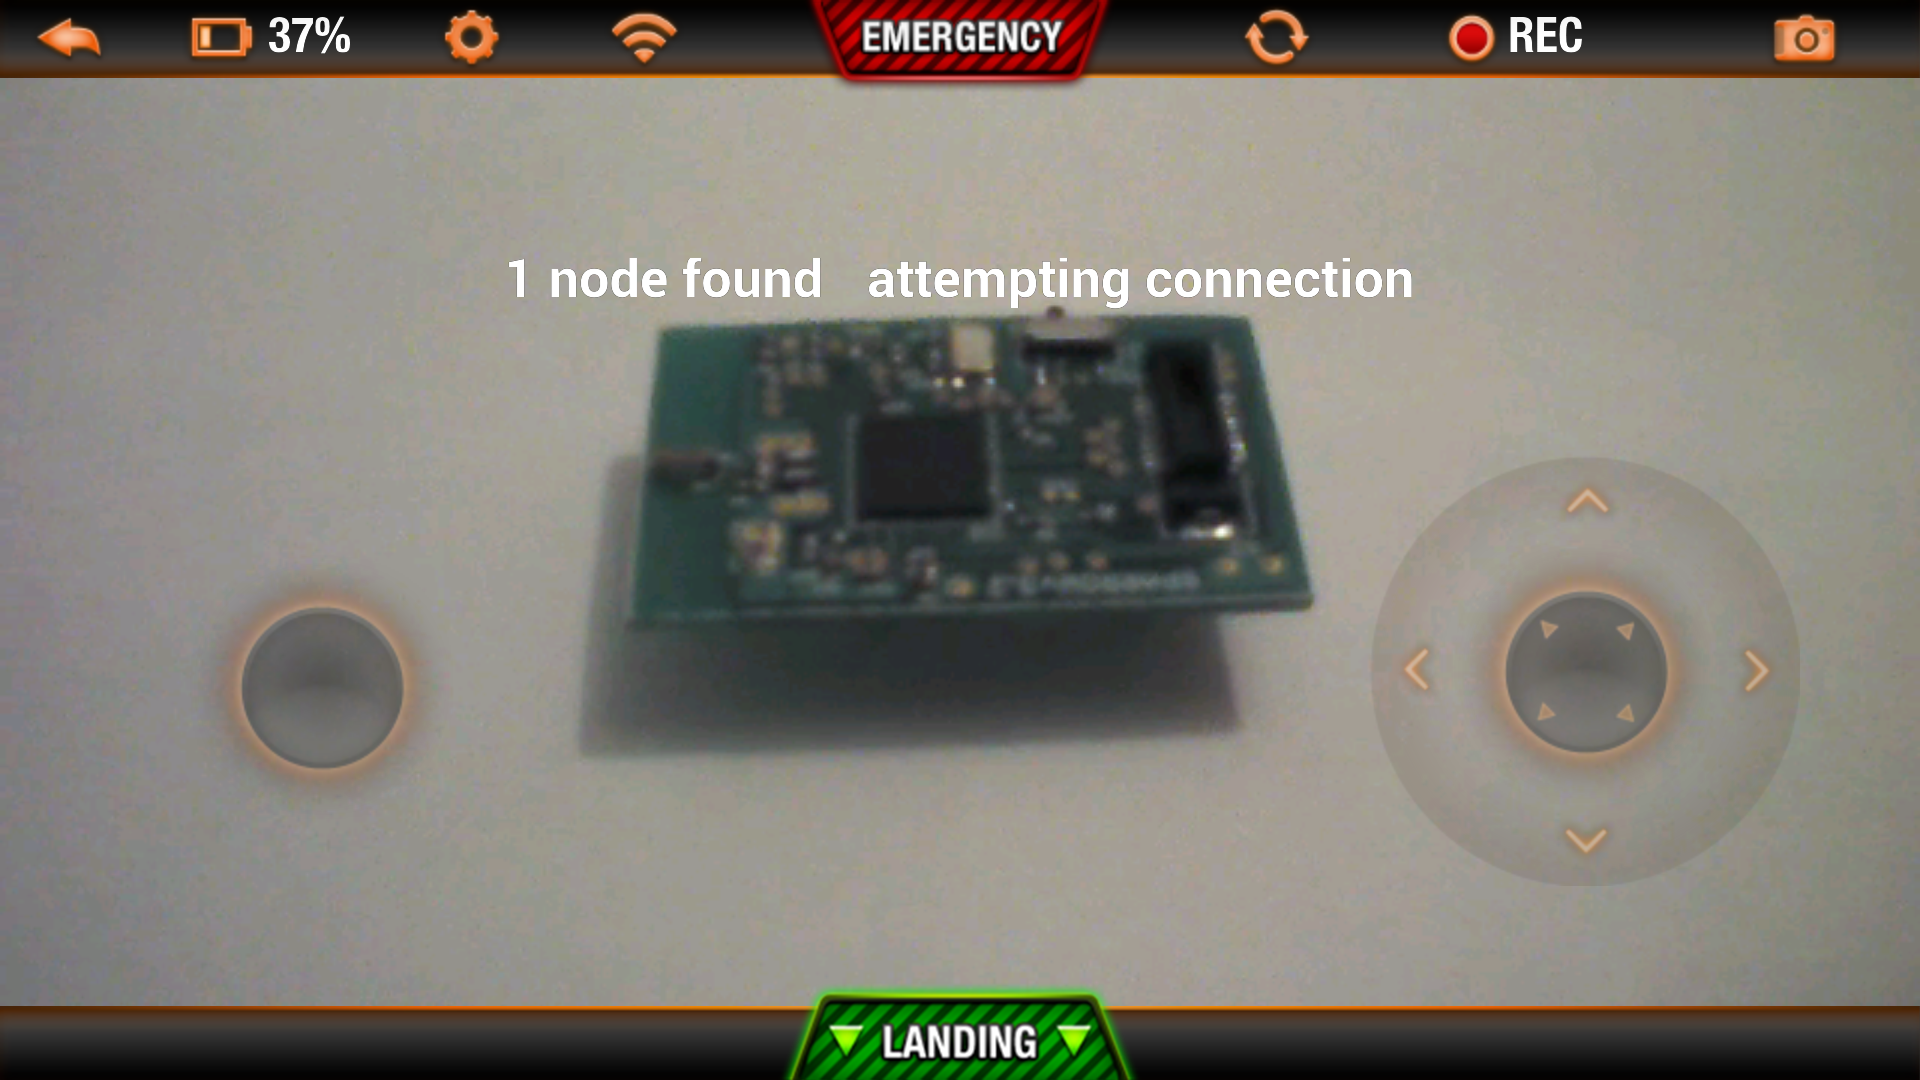
\includegraphics[width=0.6\textwidth]{img/app.png}
\caption{FreeFlight 2.0 with added WSN capabilities } \end{figure*}
 



